\documentclass[letterpaper]{jpconf}
\usepackage{graphicx}
\usepackage{subfigure}
\usepackage{url}
\usepackage{iopams}
\usepackage[pdftex,
      colorlinks=true,
      urlcolor=blue,       % \href{...}{...} external (URL)
      filecolor=green,     % \href{...} local file
      linkcolor=blue,       % \ref{...} and \pageref{...}
      pagebackref,
      pdfpagemode=UseNone,
      bookmarksopen=true]{hyperref}


\begin{document}
% paper title
\title{Many-core applications to online track reconstruction in HEP experiments}
% Author list
\author{S.~Amerio$^1$, 
  D.~Bastieri$^1$, 
  M.~Corvo$^1$, 
  A.~Gianelle$^1$, 
  W.~Ketchum$^2$,
  T.~Liu$^3$, 
  A.~Lonardo$^4$, 
  D.~Lucchesi$^1$,
  S.~Poprocki$^5$, 
  R.~Rivera$^3$, 
  L.~Tosoratto$^4$,
  P.~Vicini$^4$
  and 
  P.~Wittich$^5$,
}
\address{$^1$ INFN and University of Padova, Italy}
\address{$^2$ Los Alamos National Laboratory, New Mexico, USA}
\address{$^3$ Fermi National Accelerator Laboratory, Illinois, USA}
\address{$^4$ INFN Roma, Italy}
\address{$^5$ Cornell University, New York, USA}

\ead{silvia.amerio@pd.infn.it}

\begin{abstract}
  In this paper we describe updates to a previous study of latencies
  in GPU for potential trigger applications, where we measured the
  latency to transfer data to/from the GPU, exploring the timing of
  different I/O technologies on different GPU models.  Those studies,
  where a simplified track fitting algorithm was parallelized and run
  on a GPU, show that latencies of few tens of microseconds can be
  achieved to transfer and process packets of 4 kB of data, combining
  the modern Infiniband data transfer technology with direct access to
  GPU memory allowed by NVIDIA GPUDirect utilities.  We now have
  expanded our latency studies to include other multi-core systems
  (Intel Xeon Phi in addition to NVIDIA GPUs). We also discuss the
  implementation of a scaled-up version of the algorithm used at CDF
  for online track reconstruction - the SVT algorithm - as a realistic
  test-case for low-latency trigger systems using new computing
  architectures for LHC experiment.

\end{abstract}

\section{Introduction}
%%% Verbatim from NSS paper
Real-time event reconstruction plays a fundamental role in High Energy
Physics (HEP) experiments at hadron colliders.  Reducing the rate of
data to be saved on tape from millions to hundreds of events per
second is critical. To increase the purity of the collected samples,
rate reduction has to be coupled with an initial selection of the most
interesting events.  In a typical hadron collider experiment, the
event rate has to be reduced from tens of MHz to a few kHz.  The
selection system (trigger) is usually organized in multiple levels,
each capable of performing a finer selection on more complex physics
objects describing the event. Trigger systems usually comprise a first
level based on custom hardware, followed by one or two levels usually
based on farms of general purpose processors.  The possibility of also
using commercial devices at a low trigger level is very appealing:
they are subject to continuous performance improvements driven by the
consumer market, are less expensive than dedicated hardware, and are
easier to support.  Among the commercial devices, Graphic Processing
Units (GPUs) are of particular interest for online selections given
their impressive computing power (the latest NVIDIA~\cite{bib_nvidia}
GPU architecture, Kepler, exceeds Teraflop computing power); moreover,
high-level programming architectures based on C/C++ such as
\textsc{cuda} and \textsc{opencl} make these devices more accessible
to the general user.  
The ultimate goal of this study is to investigate the strengths and weaknesses
of GPUs when applied in a low latency environment, with particular
emphasis on the data transfer latency to/from the GPU and the
algorithm latency for processing on the GPU in a manner similar to a
typical HEP trigger application.

We showed initial studies on GPU performance in low-latency
environments ($\sim$100\,$\mu$s) in a previous paper~\cite{TIPP2011,NSS2012}.  In this paper we extend those studies measuring the
timing performance of different GPU cards in different data I/O
environments. The algorithm run on the GPU is a complete version of
the fast track fitting algorithm of the Silicon Vertex Tracker (SVT)
system at CDF~\cite{SVT1}. 
%We also compare the performance of GPU
%cards from different manufacturers (AMD vs NVIDIA) and different
%computing environments (\textsc{cuda} and \textsc{opencl}) on the same
%card. 
One of the goals of the studies is to explore using a concrete
algorithm what gains one can achieve with varying degrees of changes
to the existing algorithm. Starting with a serial algorithm
implemented on a CPU, we test an \textit{embarrassingly parallel} algorithm
on the Intel MIC environment. In this case each event is handled
independently by a core on the accelerator, and the parallelization is
achieved with only minor changes to the legacy code and is only
possible in the Intel MIC environment. Next we consider an algorithm
where we unroll three internal nested loops and run these in parallel
on a GPU, using the \textsc{cuda}~\ref{bib_cuda} environment. This second 
approach is programmatically more complicated and less trivial to implement. In
neither case have we re-thought the basic algorithms or the data
structures used. To achieve optimal performance, these steps would
have to be taken.  As one might expect, the improvement from the first
approach is rather modest, and the second approach shows larger
performance gains.

\section{SVT track fitting algorithm}
The Silicon Vertex Trigger (SVT)~\cite{SVT1,SVT2} is a 
track reconstruction processor used at 
trigger level in the CDF experiment at Tevatron accelerator. It reconstructs 
tracks in about 20 $\mu s$ in time in two steps: for each event 
first low resolution tracks (\textit{roads}) are found among the hits left 
in the tracking detector by charged particles; then track fitting is 
performed on all possible combinations of hits inside a road. 
This algorithm uses a linearized approximation to track-fitting as 
implemented in hardware (described in greater detail in~\cite{SVT3}). 
With the SVT approach, the determination of the track parameters 
($p_i$) is reduced to a simple scalar product:
\[
p_i = \vec{f_i} \cdot \vec{x_i} + q_i,
\]
where $\vec{x_i}$ are input silicon hits, and $\vec{f_i}$ and $q_i$ are 
pre-defined constant sets. For each set of hits, the algorithm
computes the impact parameter $d_0$, the azimuthal angle $\phi$, 
the transverse momentum $p_\mathrm{T}$ , and the $\chi^2$ of the
fitted track by using simple operations such as memory lookup and 
integer addition and multiplication.

We ported the track fitting part to parallel devices, as it is well suited to 
be parallelized. 

\subsection{Code implementation}
The starting point of of our studies is the SVT track fitting simulation code, 
written in C language. SVT track fitting is divided into three main functions: 
first the unpacking of input data and filling of all the necessary arrays, 
followed by the computation of all possible combinations of hits in each road 
and finally the fit on each combination. Three main loops are 
present - on events, roads and hit combinations. 
To be run on GPUs, the code has been ported to \textsc{cuda}: each step - 
unpack, combine and track fit - is performed by a specific kernel;
the three nested loops are unrolled so that each GPU thread processes a 
single combination of hits. 
To run on MIC, we adopted the so-called \textit{embarrassingly parallel} 
approach and used pragma OpenMP for statements to unroll the external loop 
on the events, so that each core processes a single event: the porting 
requires much less effort compared to CUDA, but the level of parallelism is 
limited.

\section{Experimental setup and data flow}
The many-core devices used in this study are listed in Table~\ref{tab_hwspecs}.

\begin{table}[!t]
  \centering
  \begin{tabular}{|l|c|c|c|c|}
    \hline
    Model & Tesla M2050 & Tesla K20m & GeForce GTX  Titan & MIC 5110P \\
    \hline
    \hline
    Performance (SP, GFlops) & 1030 & 3520 & 4500 & 2022 \\
    Memory bandwidth  (GB/s) & 148 & 208 & 288  & 320\\   
    Memory size (GB) & 3 & 5 & 6 & 8 \\
    Number of cores & 448 & 2496 & 2688 & 240 \\
    Clock speed (GHz) & 1.15 & 0.706 & 0.837 & 1.053 \\
    \hline
  \end{tabular}
  \caption{Capabilities of the many-core devices used in this study, according to the manufacturer's specifications.}
  \label{tab_hwspecs}
\end{table}

To measure the data transfer latency we use a computing cluster composed of 
12 identical nodes.  Each node contains a Intel Xeon E6520 2.4 GHz 
CPU and two Tesla M2075 GPU cards. The nodes are connected by InfiniBand 
communication links using Connect-X2 Mellanox or Apenet+ adapters. 
Apenet+ is an FPGA-based PCIe board supporting peer-to-peer communication with 
Tesla and Kepler cards~\cite{apenet2010}.
Two nodes of this cluster are used to measure data transfer latency,
one acting as a transmitter and the
other as a receiver.  Data are transferred from the transmitter to the 
receiver, processed on the GPU and sent back to the receiver (see
Fig.~\ref{fig_data_flow}).  
The latency for a complete loop is measured on the transmitter using 
standard C libraries.

\begin{figure}[!h]
\centering
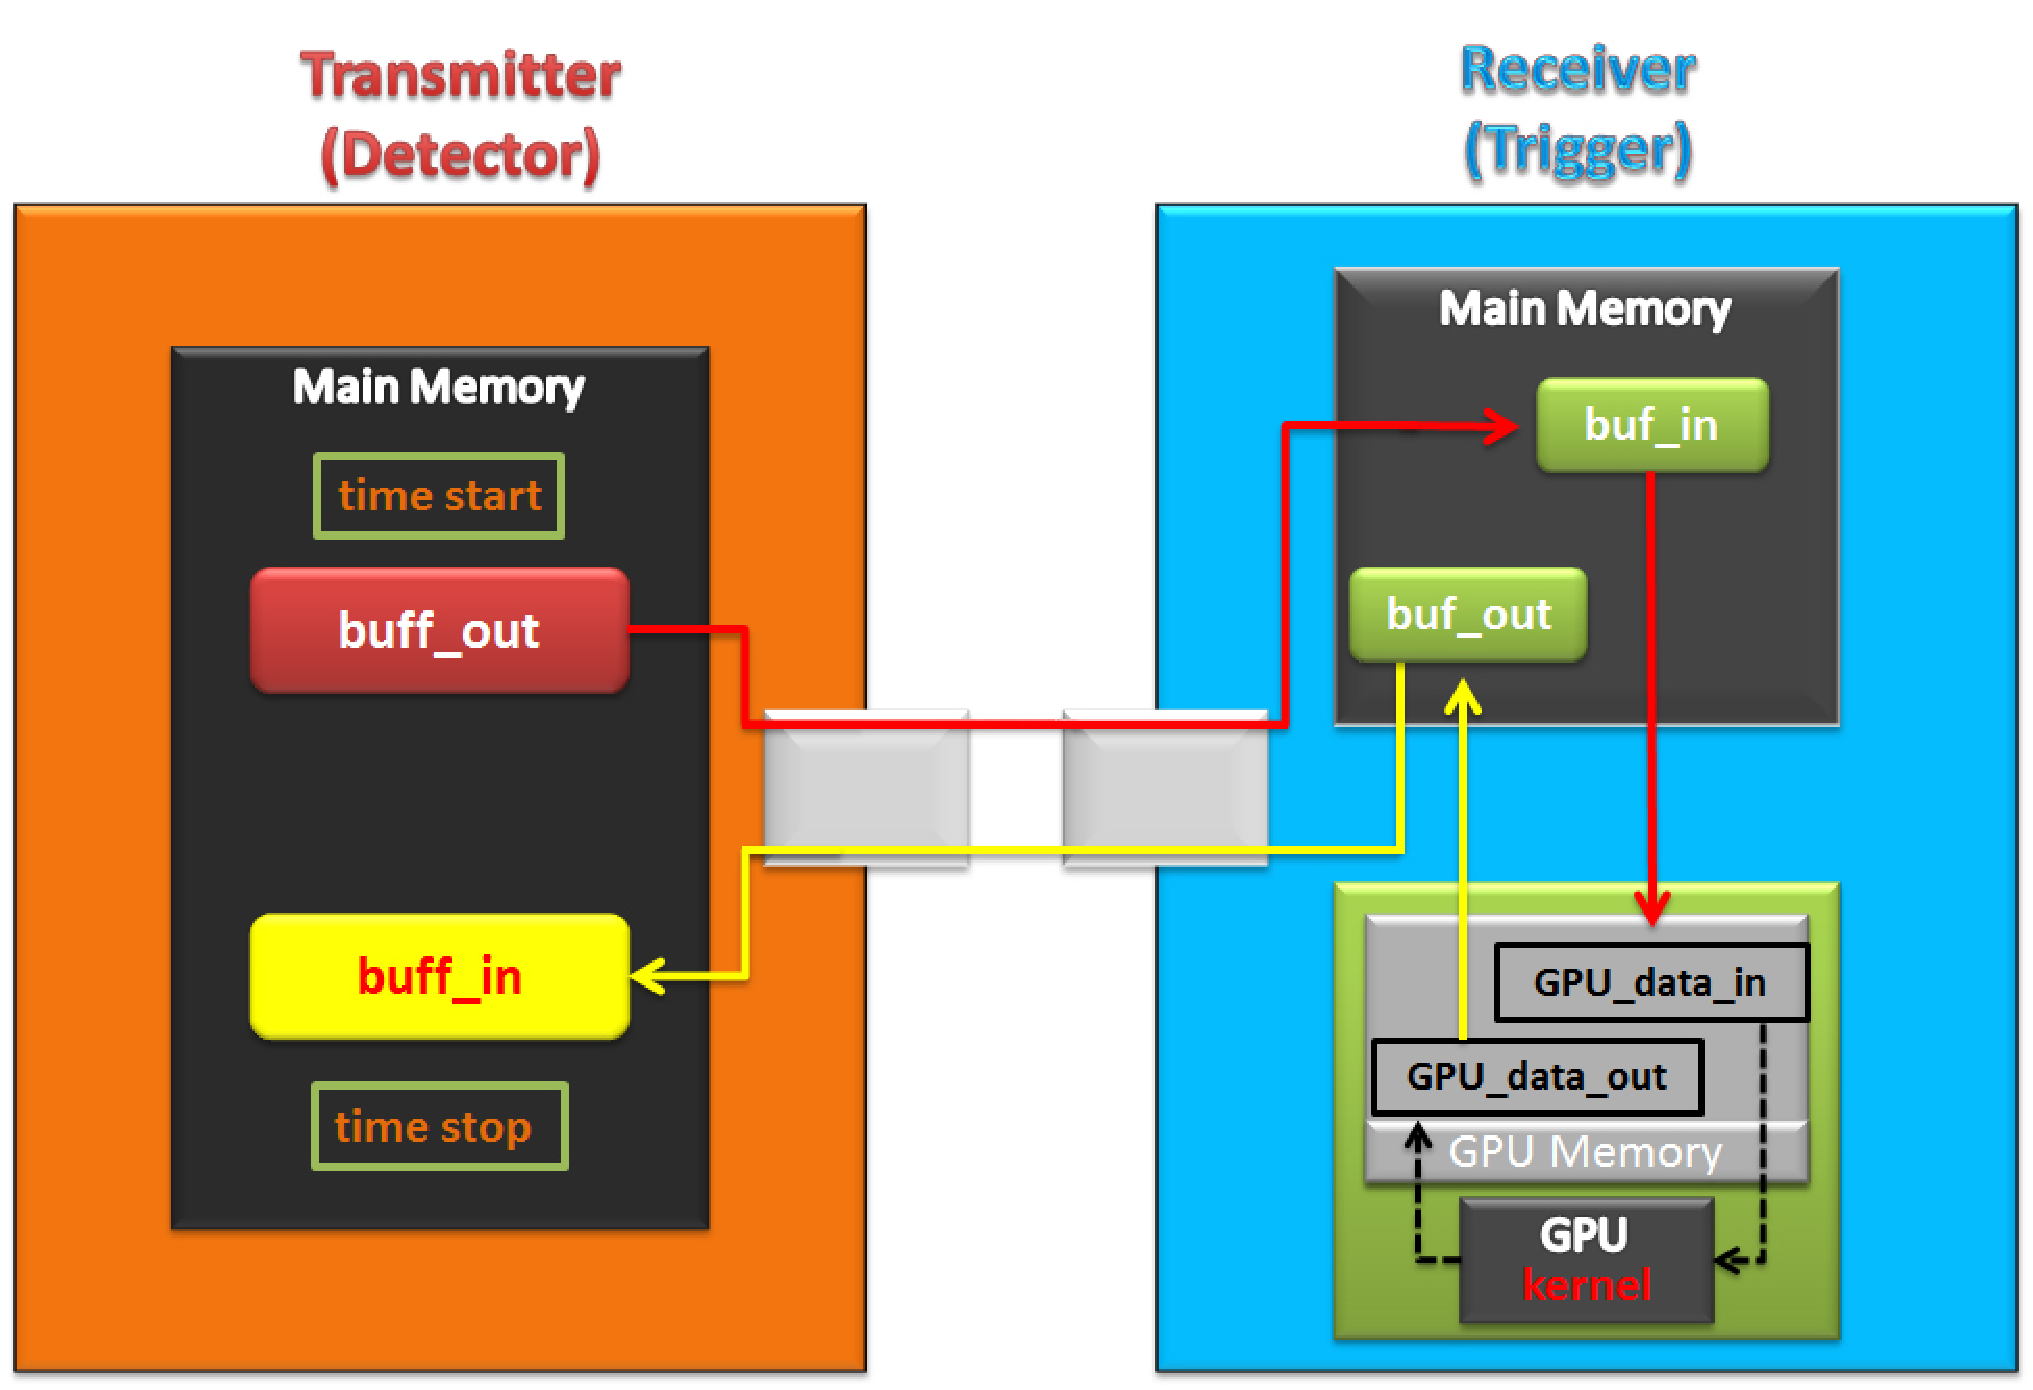
\includegraphics[width=3.5in]{figures/SetUp-general}
\caption{Data flow. Data is sent from the transmitter PC to the
  receiver PC, where it is processed by the GPU before being returned
  to the transmitter PC. The transmitter plays the role of the
  detector as the source of the data and as an upstream trigger
  processor as the data's ultimate sink. The receiver PC plays the
  role of a component in the trigger system. }
\label{fig_data_flow}
\end{figure}

In this setup, the transmitter can represent the detector, as
the source of the data, or an upstream trigger processor, as
the ultimate sink of the data, while the the receiver is the
trigger system: the time to transfer data to the receiver is thus a
rough estimate of the latency to transfer the data from the detector
front-end to the trigger system.

\section{Results}
We use as input data events with a fixed number of roads and combinations: 
each event has 2048 combinations to be fitted. To explore different data 
taking conditions the number of events ranges from one to 3000, i.e. from 2048 
to about six millions of combinations to fit.
 
\subsection{Data processing}
Each data sample is processed 100 times by the track fitting algorithm. 
The average latency as a function of the number of fits is presented in 
Fig.~\ref{fig:algo_only_timing} for the serial,
embarrassingly parallel and parallel algorithms. We see that the
embarrassingly parallel algorithm gives a modest increase with respect
to the serial (CPU) algorithm. Switching to a fully parallel algorithm
affords a much more significant speed improvement. 
Accelerators performance drop with decreasing number of fits, as can be seen 
in Fig.~\ref{fig:algo_only_timing_zoom}.
Fig.~\ref{fig:algo_only_speedup} shows the speed-up with respect to the serial 
algorithm run on a standard CPU (Intel Xeon E5630): the maximum gain is 
obtained processing at least 500 events. This means that to fully exploit 
parallel architectures millions of fits have to be performed in parallel.  


%\begin{figure*}[!t]
%\centering
%\subfigure[]
%{\label{fig:algo_only_timing}
%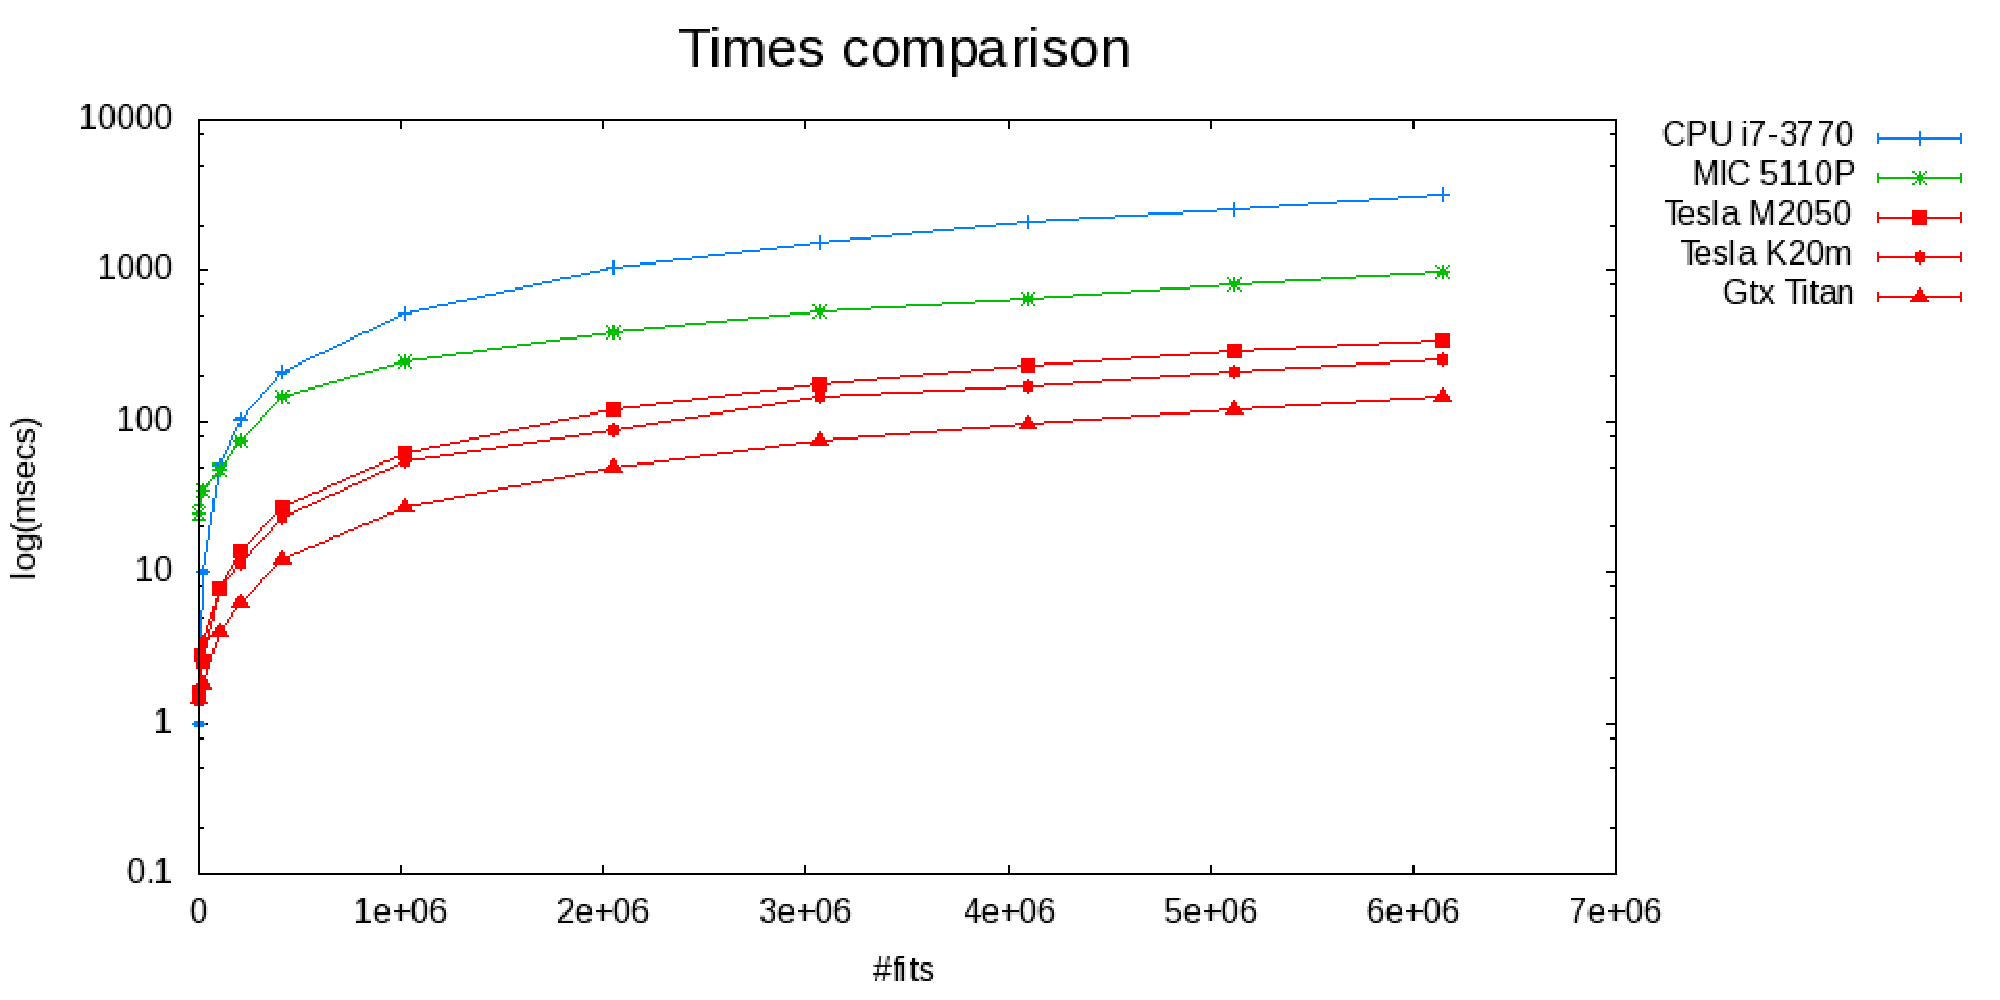
\includegraphics[width=3in]{figures/TimeComp_MIC.pdf}}
%\hspace{1mm}
%\subfigure[]
%{\label{fig_algo_only_timing_zoom}
%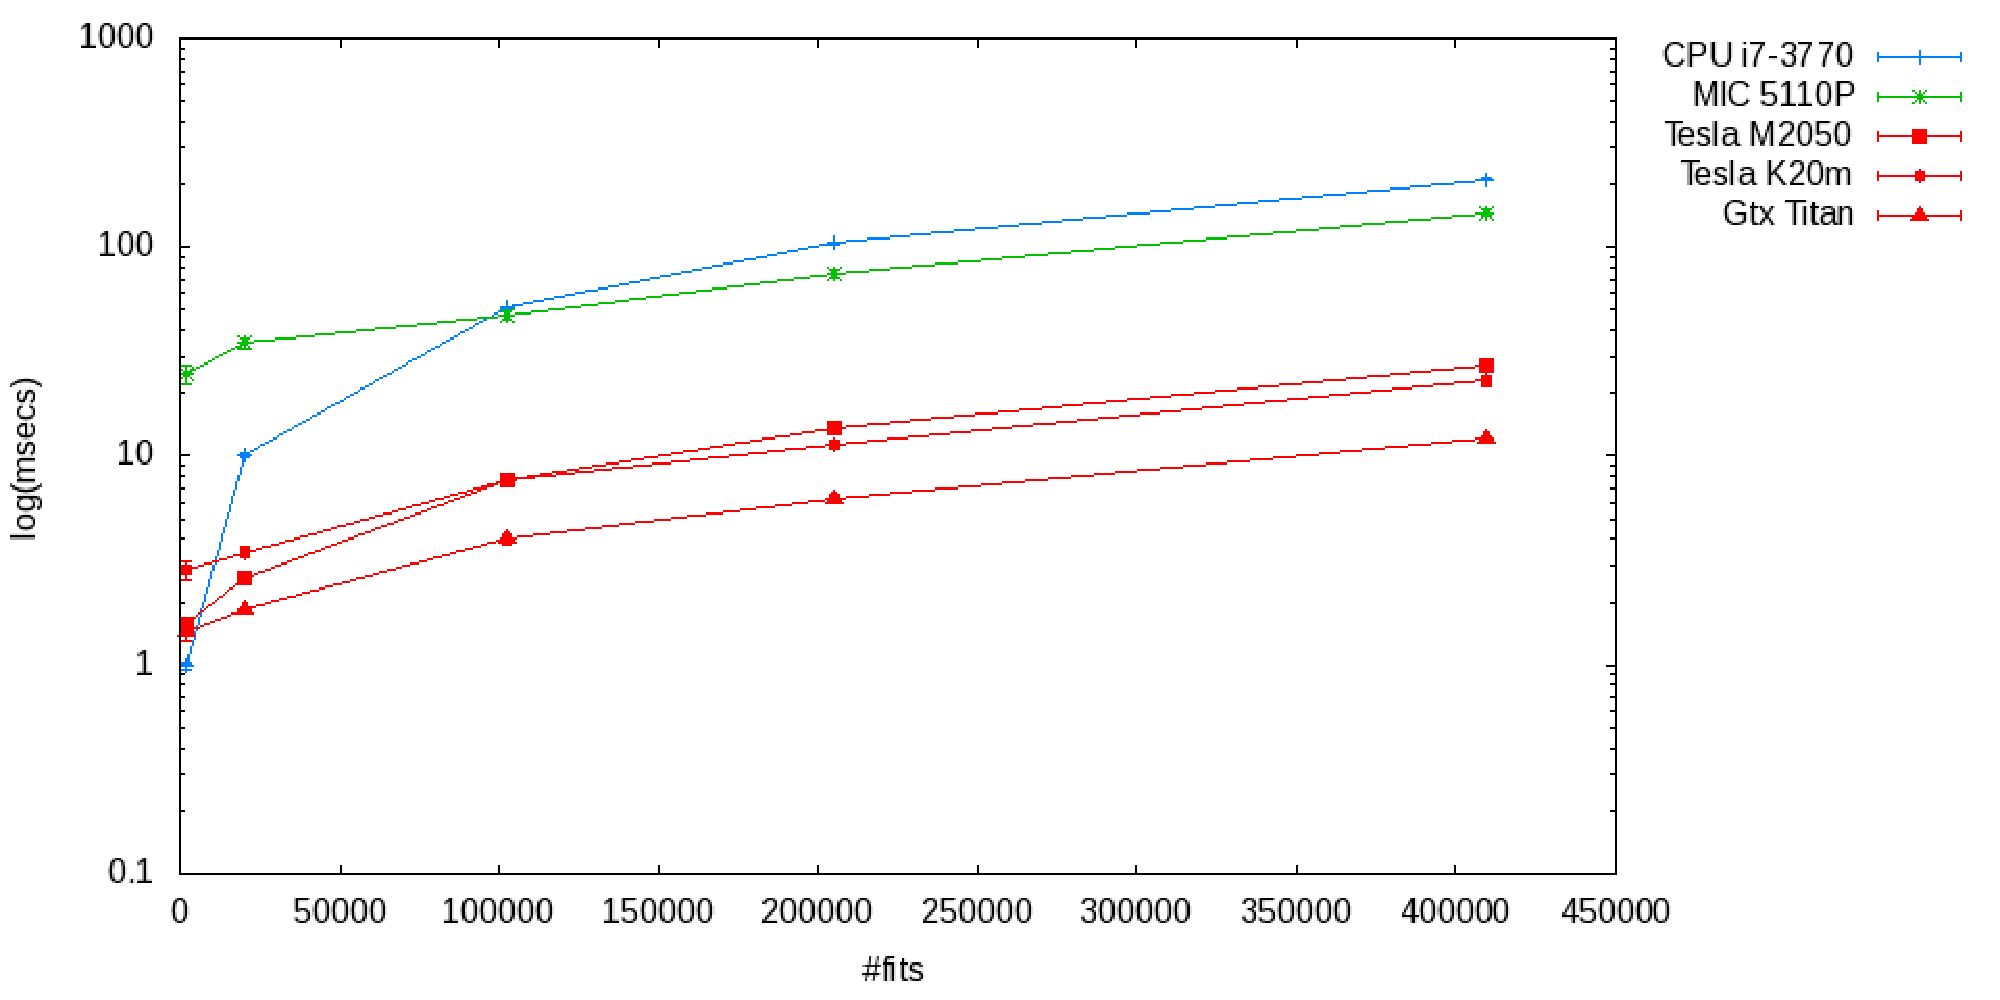
\includegraphics[width=3in]{figures/TimeCompZoom_MIC.pdf}}
%\caption{breakdown}
%\end{figure*}
%

 \begin{figure}[!tbp]
    \centering
    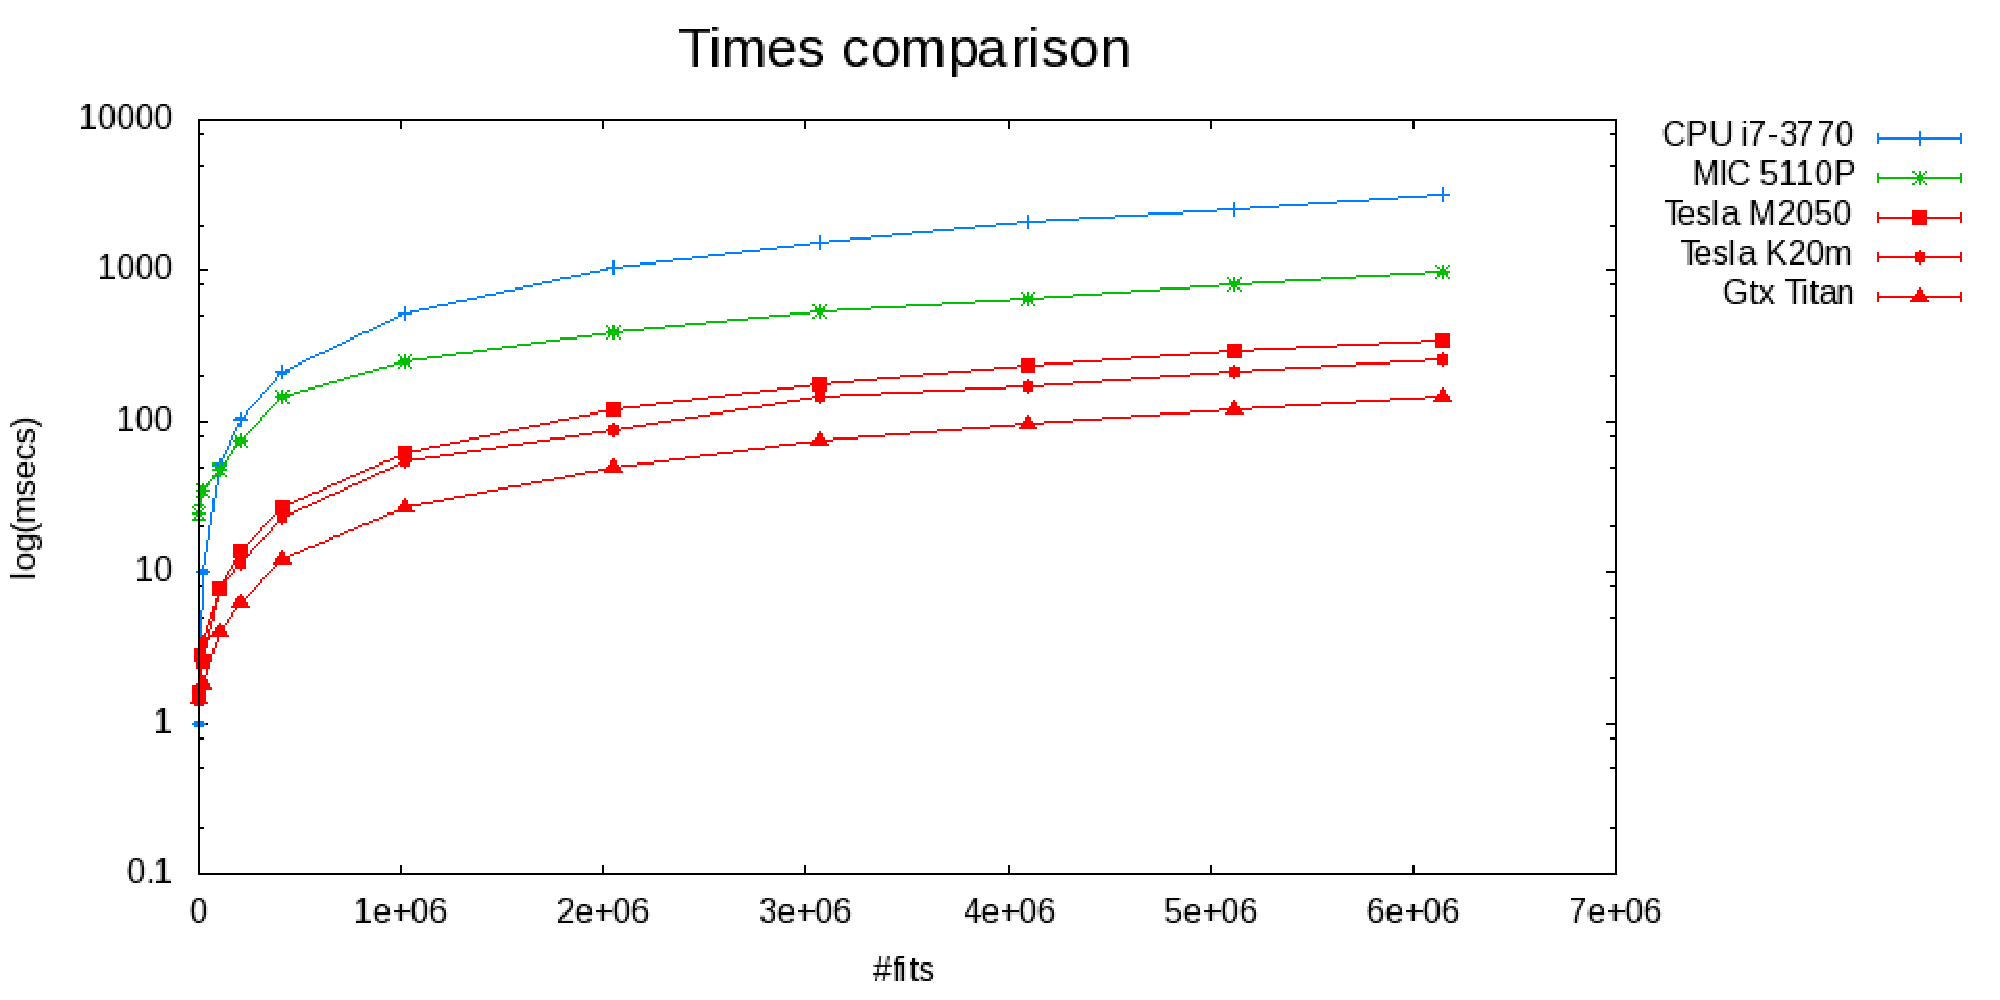
\includegraphics[width=0.9\linewidth]{figures/TimeComp_MIC.pdf}
     \caption{Algorithm-only comparison for timing as a function of the
      number of track fits. We compare timing on CPUs (serial), Xeon Phi
      (embarrassingly parallel), and GPUs (fully parallel). }
    \label{fig:algo_only_timing}
  \end{figure}
 
  \begin{figure}[!tbp]
    \centering
    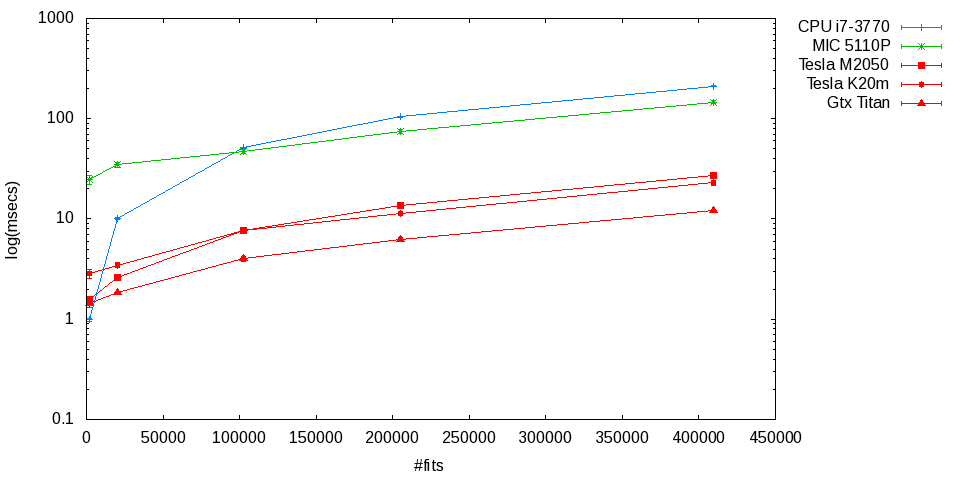
\includegraphics[width=0.9\linewidth]{figures/TimeCompZoom_MIC.png} 
    \caption{Algorithm-only comparison for timing as a function of the
      number of track fits: zoom in the low number of fits region.}
    \label{fig:algo_only_timing_zoom}
  \end{figure}
 
 \begin{figure}[!tbp]
   \centering
   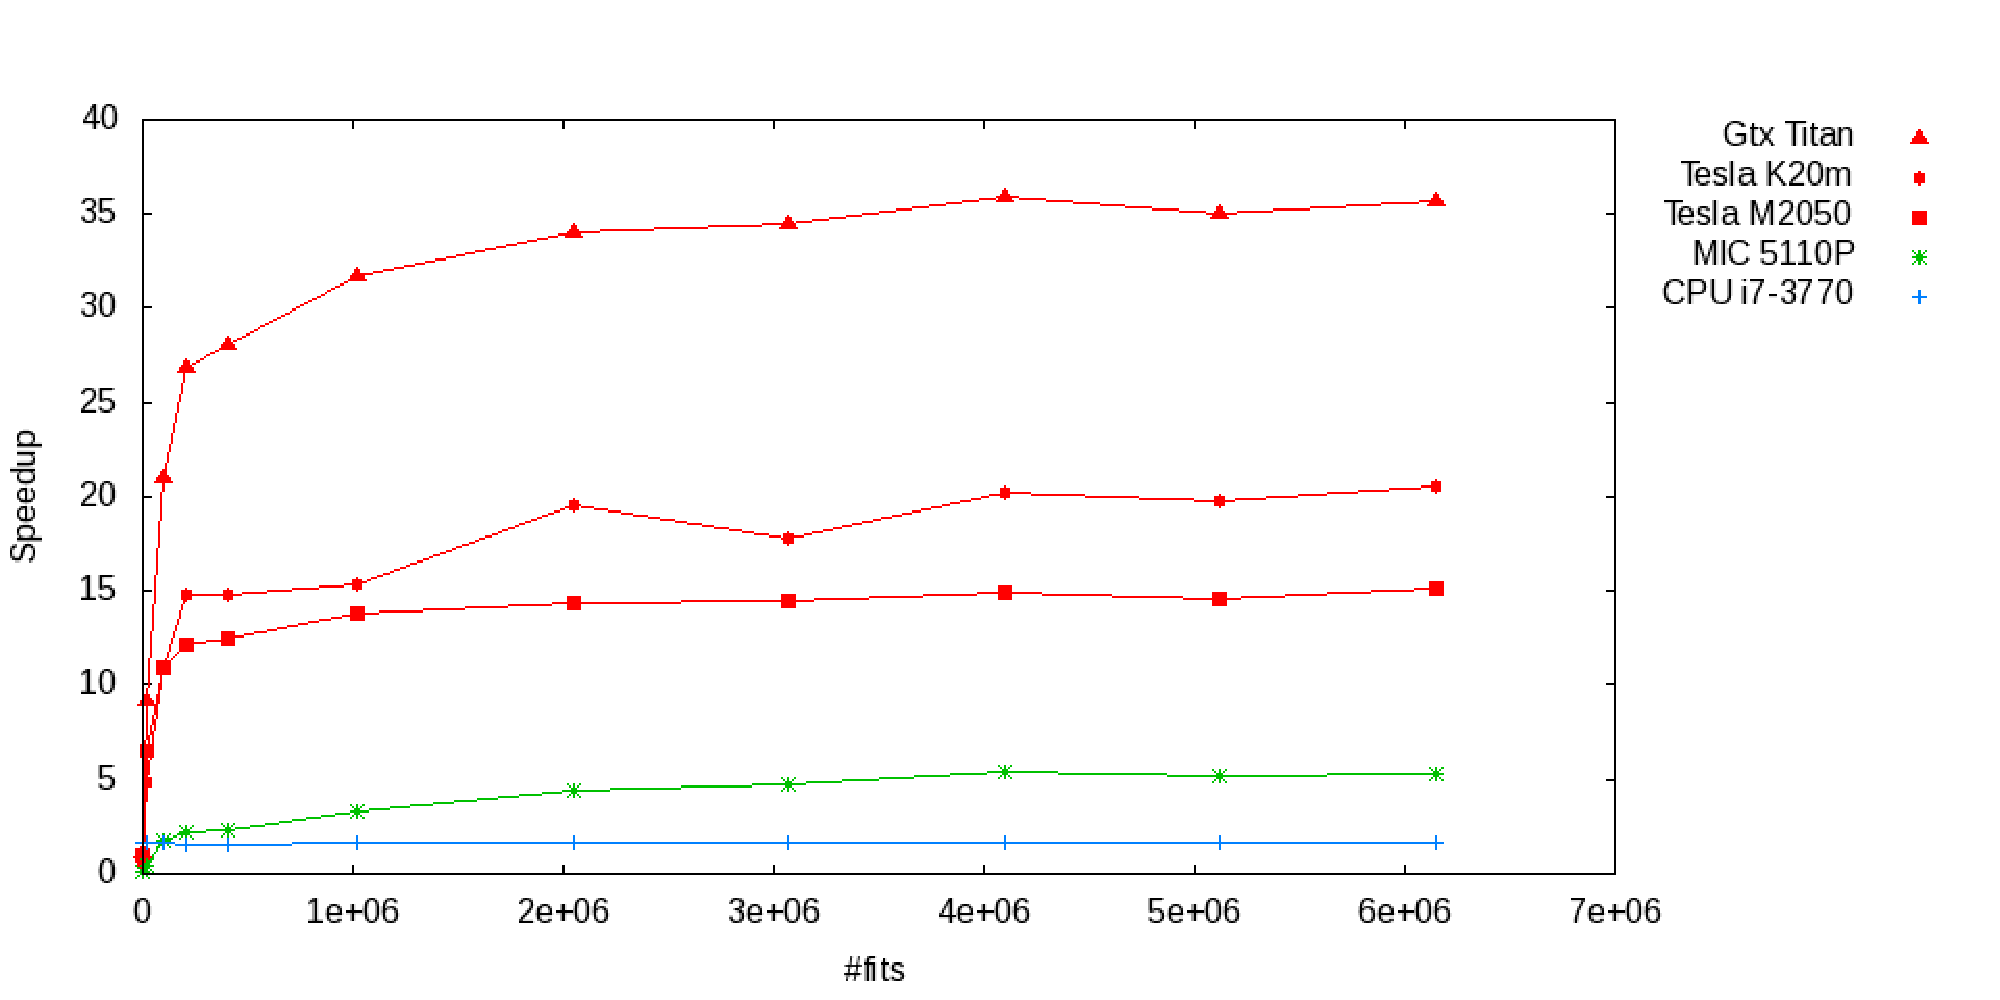
\includegraphics[width=0.9\linewidth]{figures/Speedup_MIC.pdf}
   \caption{Speed-up with respect to a standard CPU (Intel Xeon E5630) .}
   \label{fig:algo_only_speedup}
 \end{figure}


\subsubsection{Breakdown of computing time}
In Fig.~\ref{fig:breakdown} we show the fractional time spent in
various parts of the algorithm for the embarrassingly parallel algorithm 
(on Intel MIC) and the parallel algorithm (on NVidia Titan GPU), as a 
function of the number of fits. On both accelerator cards the fractional times
are constant over 500 input events, where computing resources are saturated. 
Differently from MIC, the fit stage takes most of the time on the GPU: this 
could be explained with the intense memory access intrinsic in 
this part of the algorithm.  


\begin{figure*}[!t]
\centering
%\subfigure[]
%{\label{fig:breakdown_CPU}
%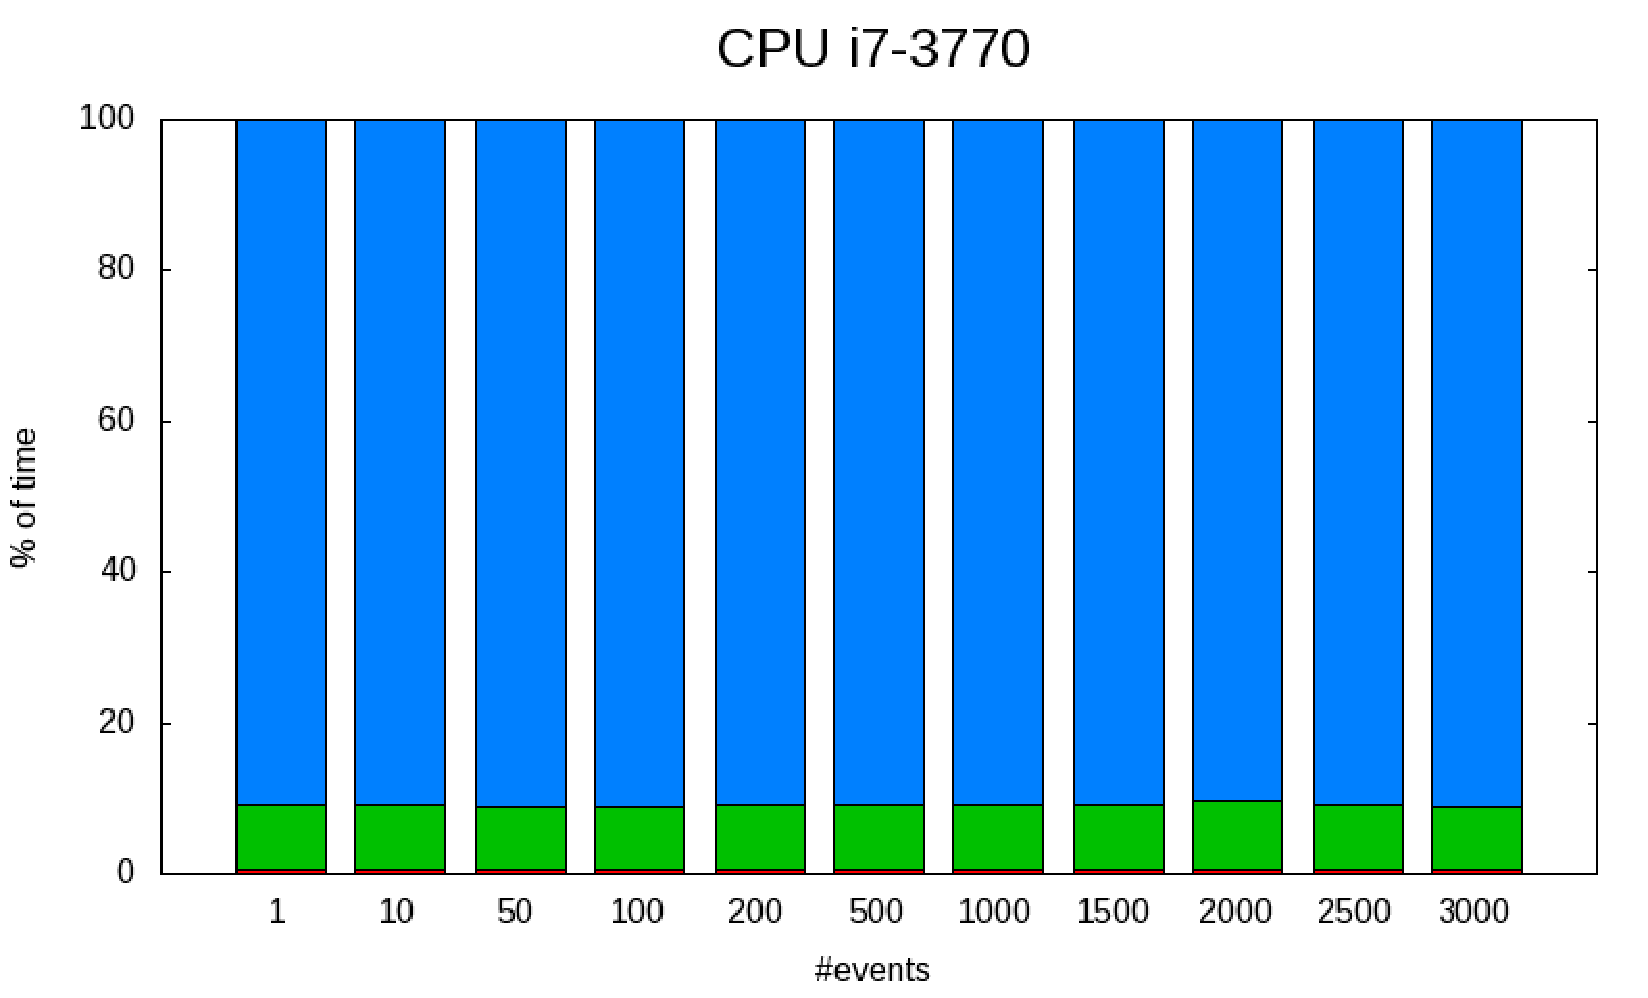
\includegraphics[width=0.4\linewidth]{figures/Cpui7_perc.pdf}}
%\hspace{1mm}
\subfigure[]
{\label{fig:breakdown_MIC}
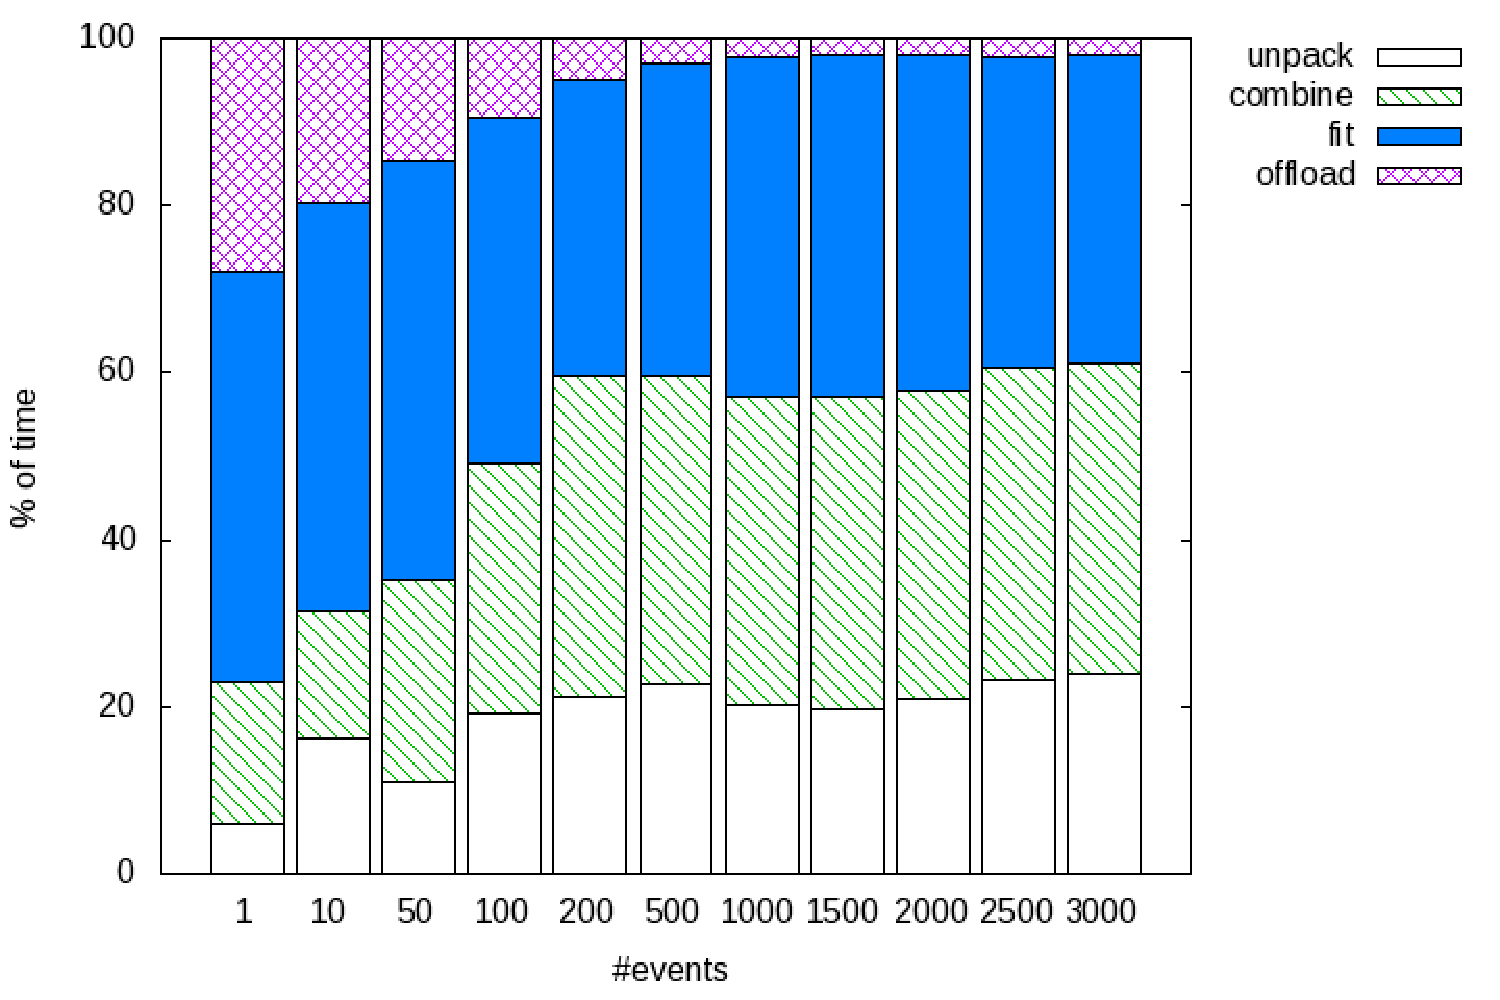
\includegraphics[width=0.45\linewidth]{figures/Mic5_perc_nk.pdf}}
\subfigure[]
{\label{fig:breakdown_GPU}
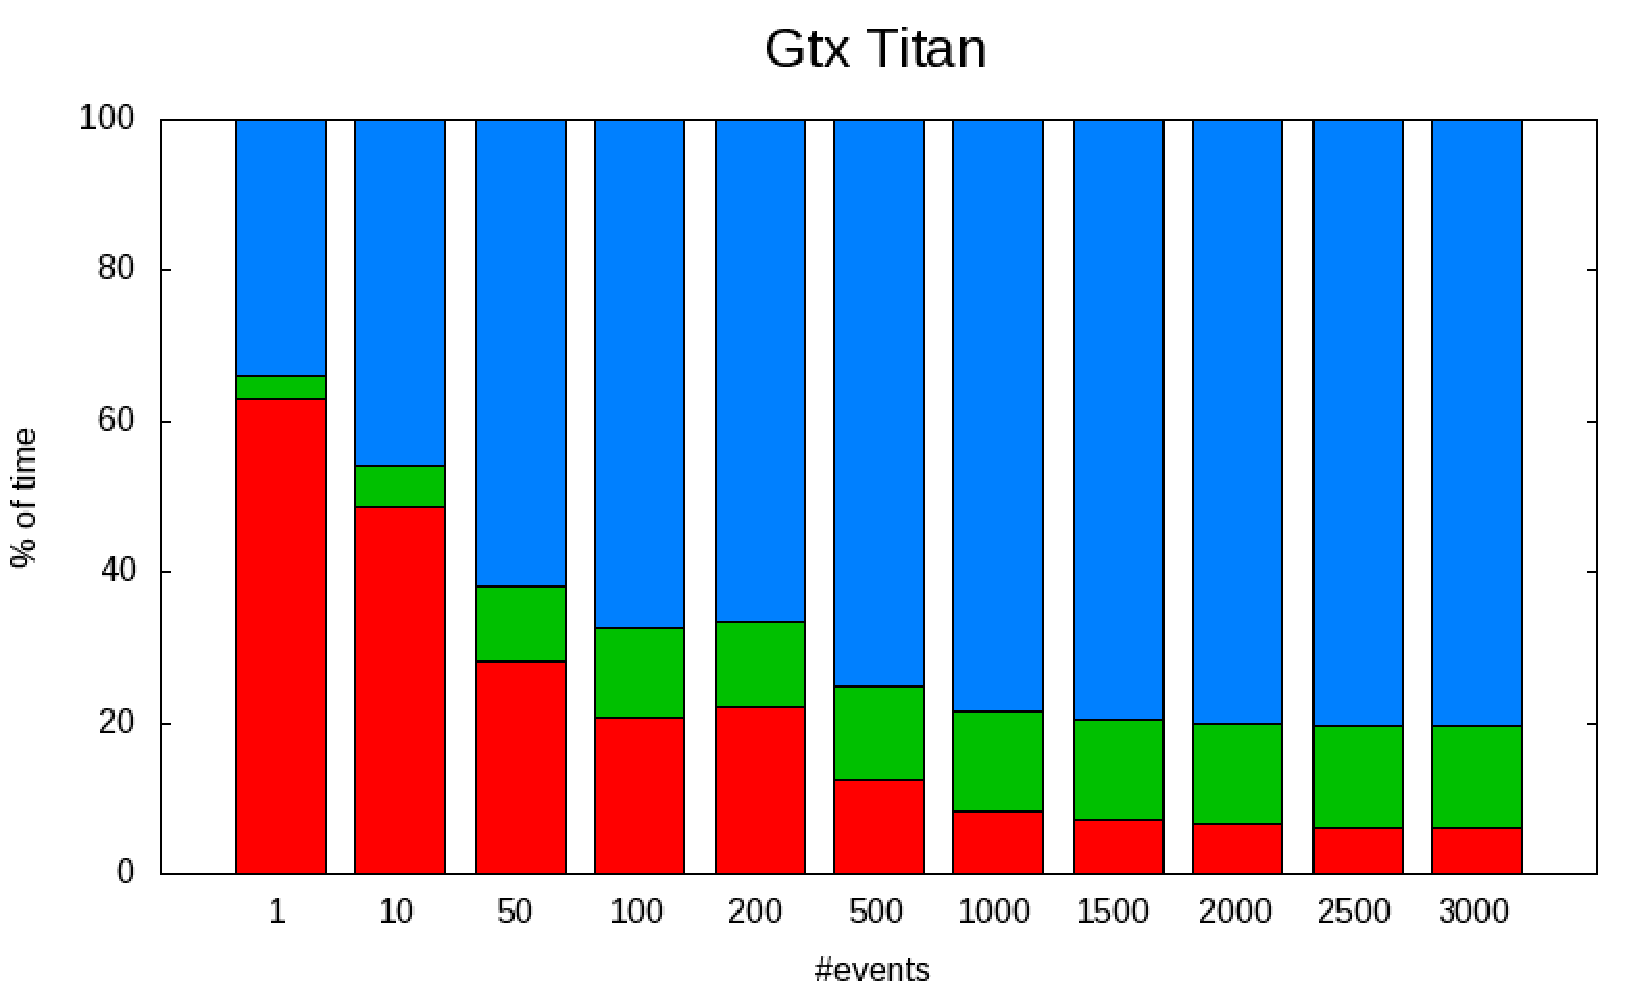
\includegraphics[width=0.45\linewidth]{figures/titan_perc.pdf}}
\caption{Breakdown of computing time.}
\end{figure*}

\subsection{Data transfer}
The experimental setup described in Fig.~\ref{fig_data_flow} allows us to 
test different data transfer  strategies to the GPU. The standard data transfer 
strategy is via the system memory, where the 
PCIe adapter card and the GPU allocate \emph{separate} buffers on the
system memory for the copy (as shown in Fig.~\ref{fig_standardDT}).
This is inefficient, as the data are copied twice in the 
system memory before being transferred to the GPU/PCIe card. 
Data may also be transferred using Direct Memory Access (DMA, 
GPUDirect\cite{bib_GPUDirect}) to the CPU memory:
the PCIe card and the GPU share the \textit{same} buffer on the CPU memory; as 
a result the data are copied only once in the CPU memory 
(Fig.~\ref{fig_GPUDirectV1}). 
With our experimental setup two additional copy strategies can be tested
which are the results of different levels of 
optimization of the GPUDirect protocol:
\begin{itemize}
\item CUDA-Aware MPI, where the copy latency is further reduced
by automatically allocating the buffer on the CPU memory;
\item peer-to-peer (P2P) strategy, when data are transferred 
directly to the GPU, without any  
intermediate copy to the CPU (Fig.~\ref{fig_GPUDirectV2}).
\end{itemize}


\begin{figure*}[!t]
\centering
\subfigure[]
{\label{fig_standardDT}
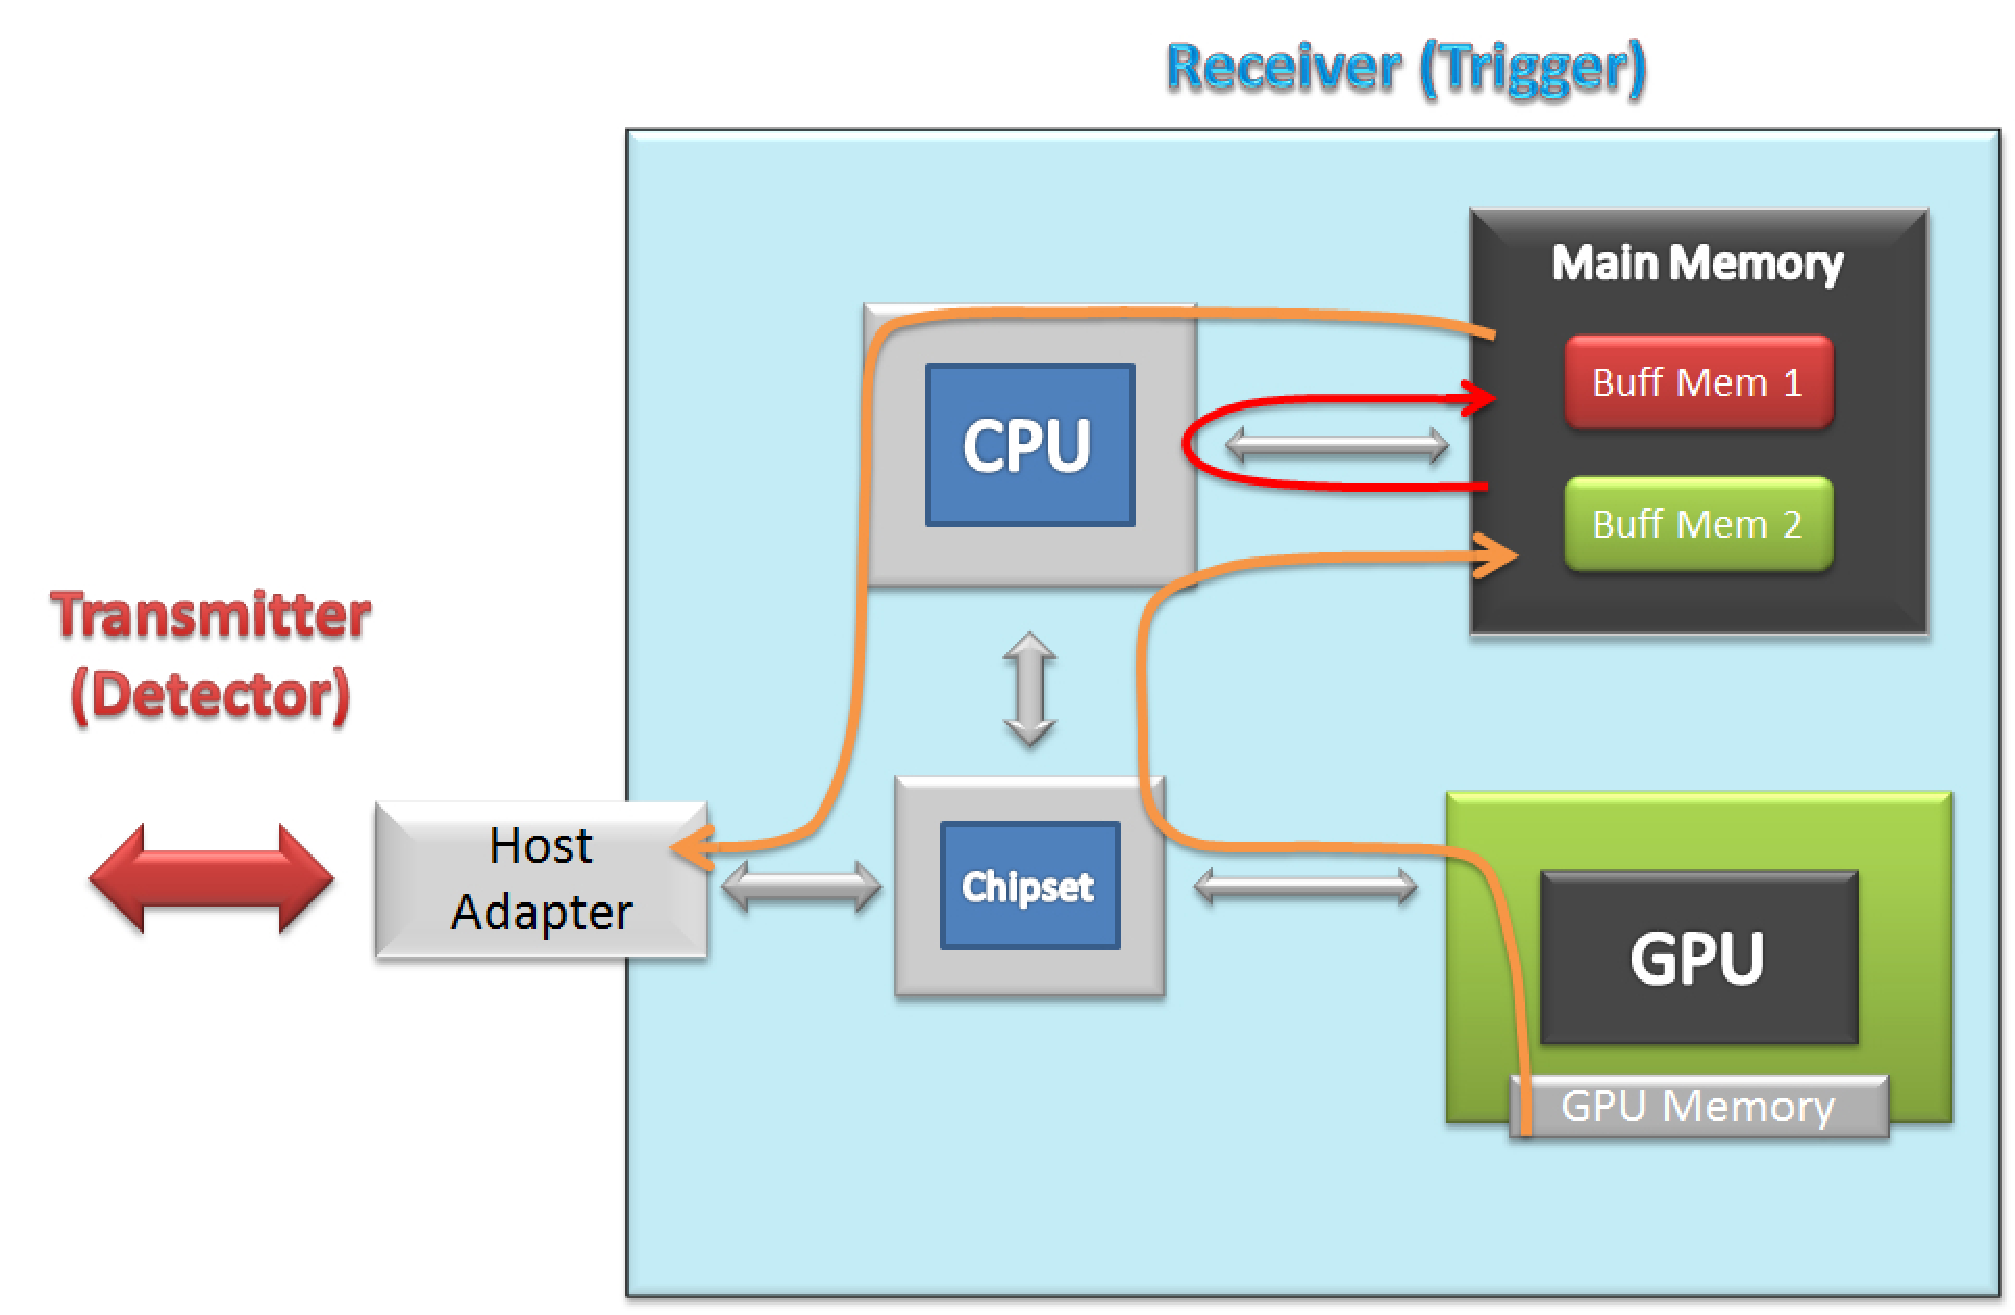
\includegraphics[width=0.3\linewidth]{figures/noGPUDirect}}
\hspace{1mm}
\subfigure[]
{\label{fig_GPUDirectV1}
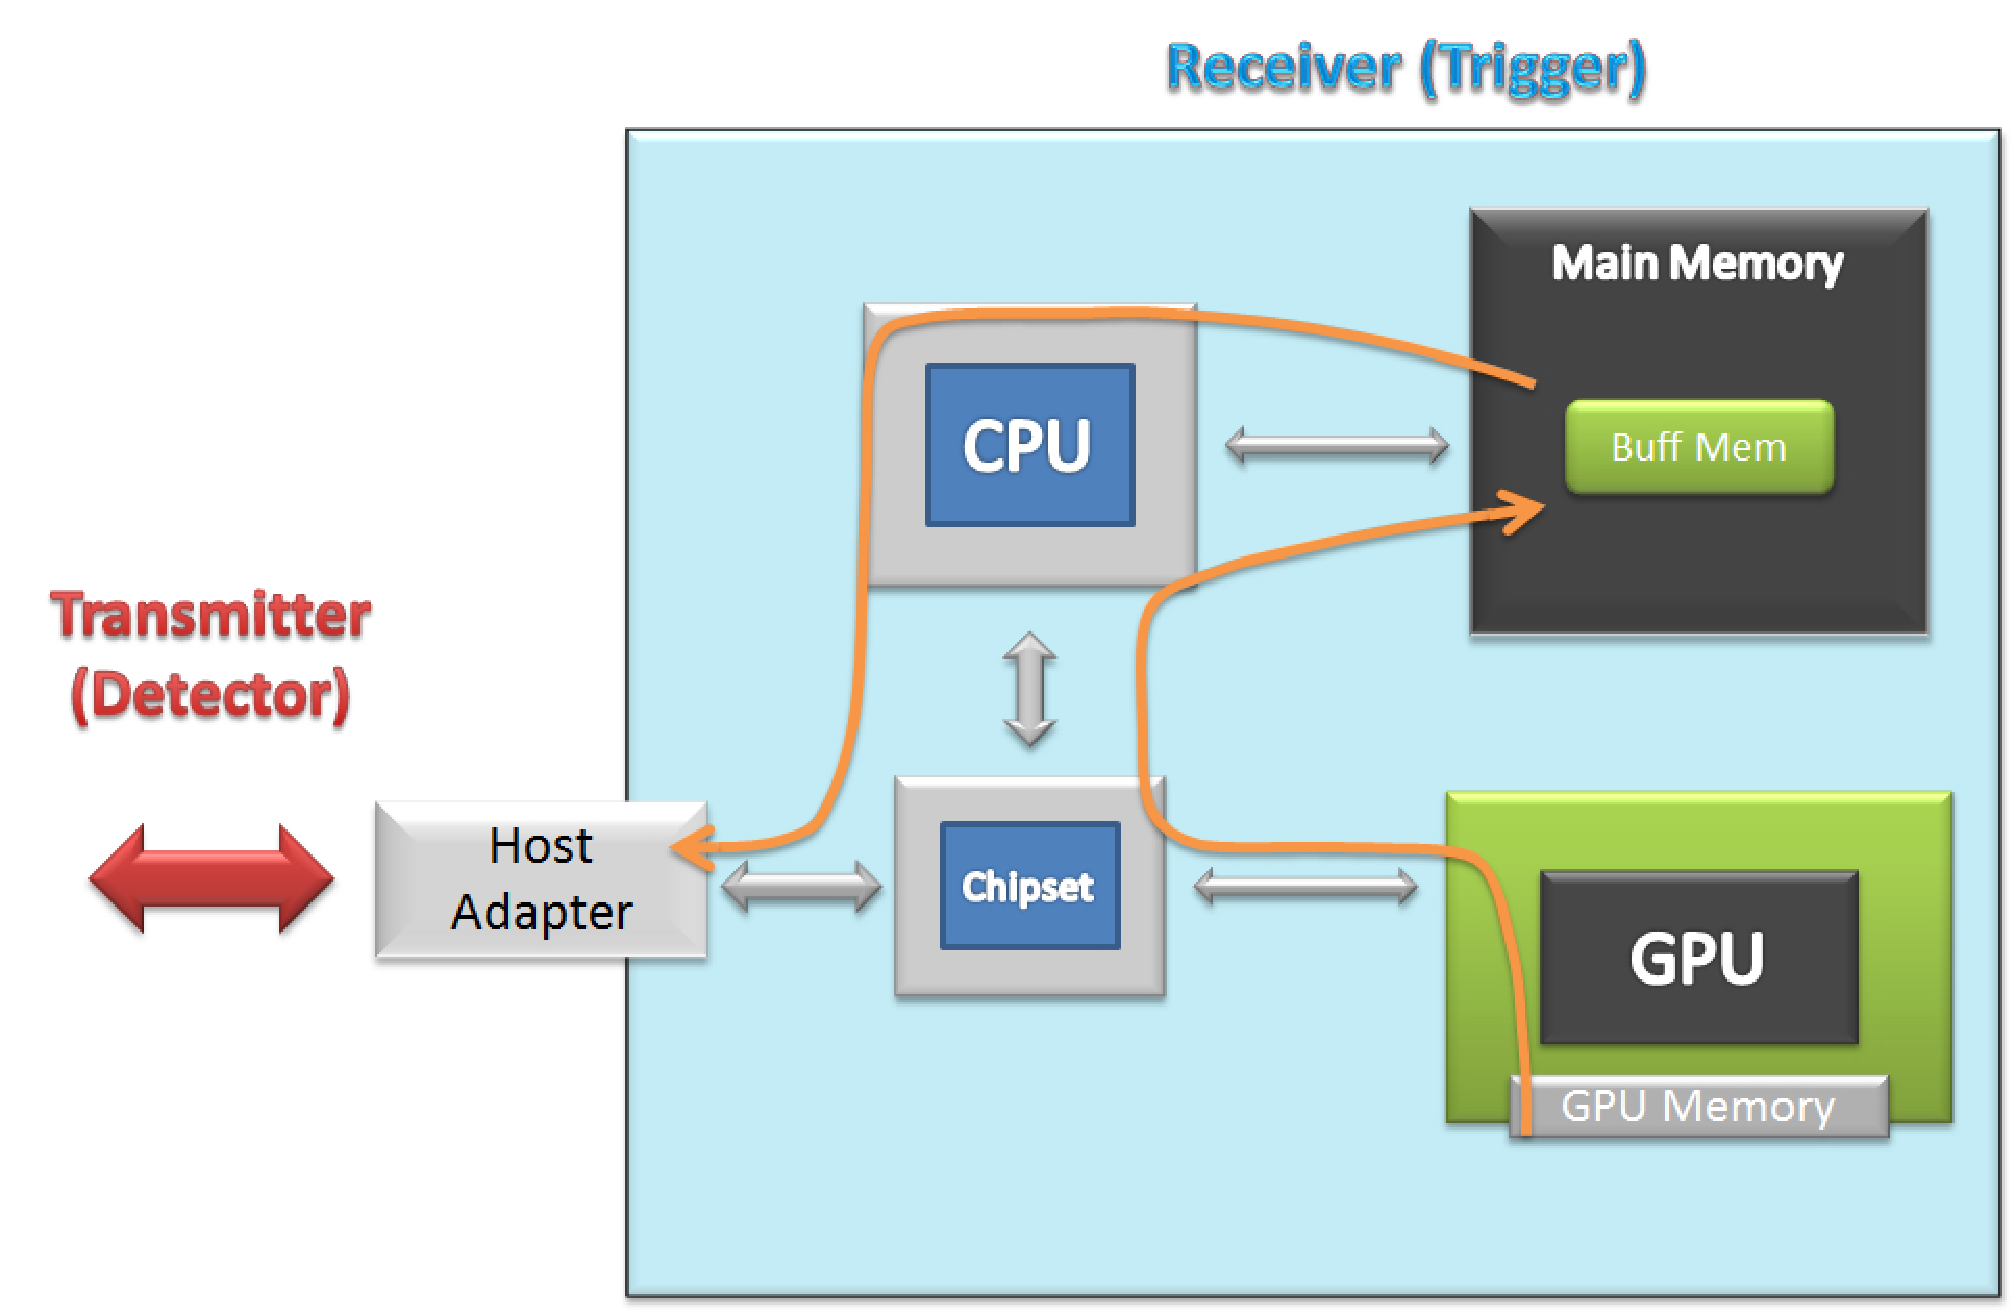
\includegraphics[width=0.3\linewidth]{figures/GPUDirect}}
\subfigure[]
{\label{fig_GPUDirectV2}
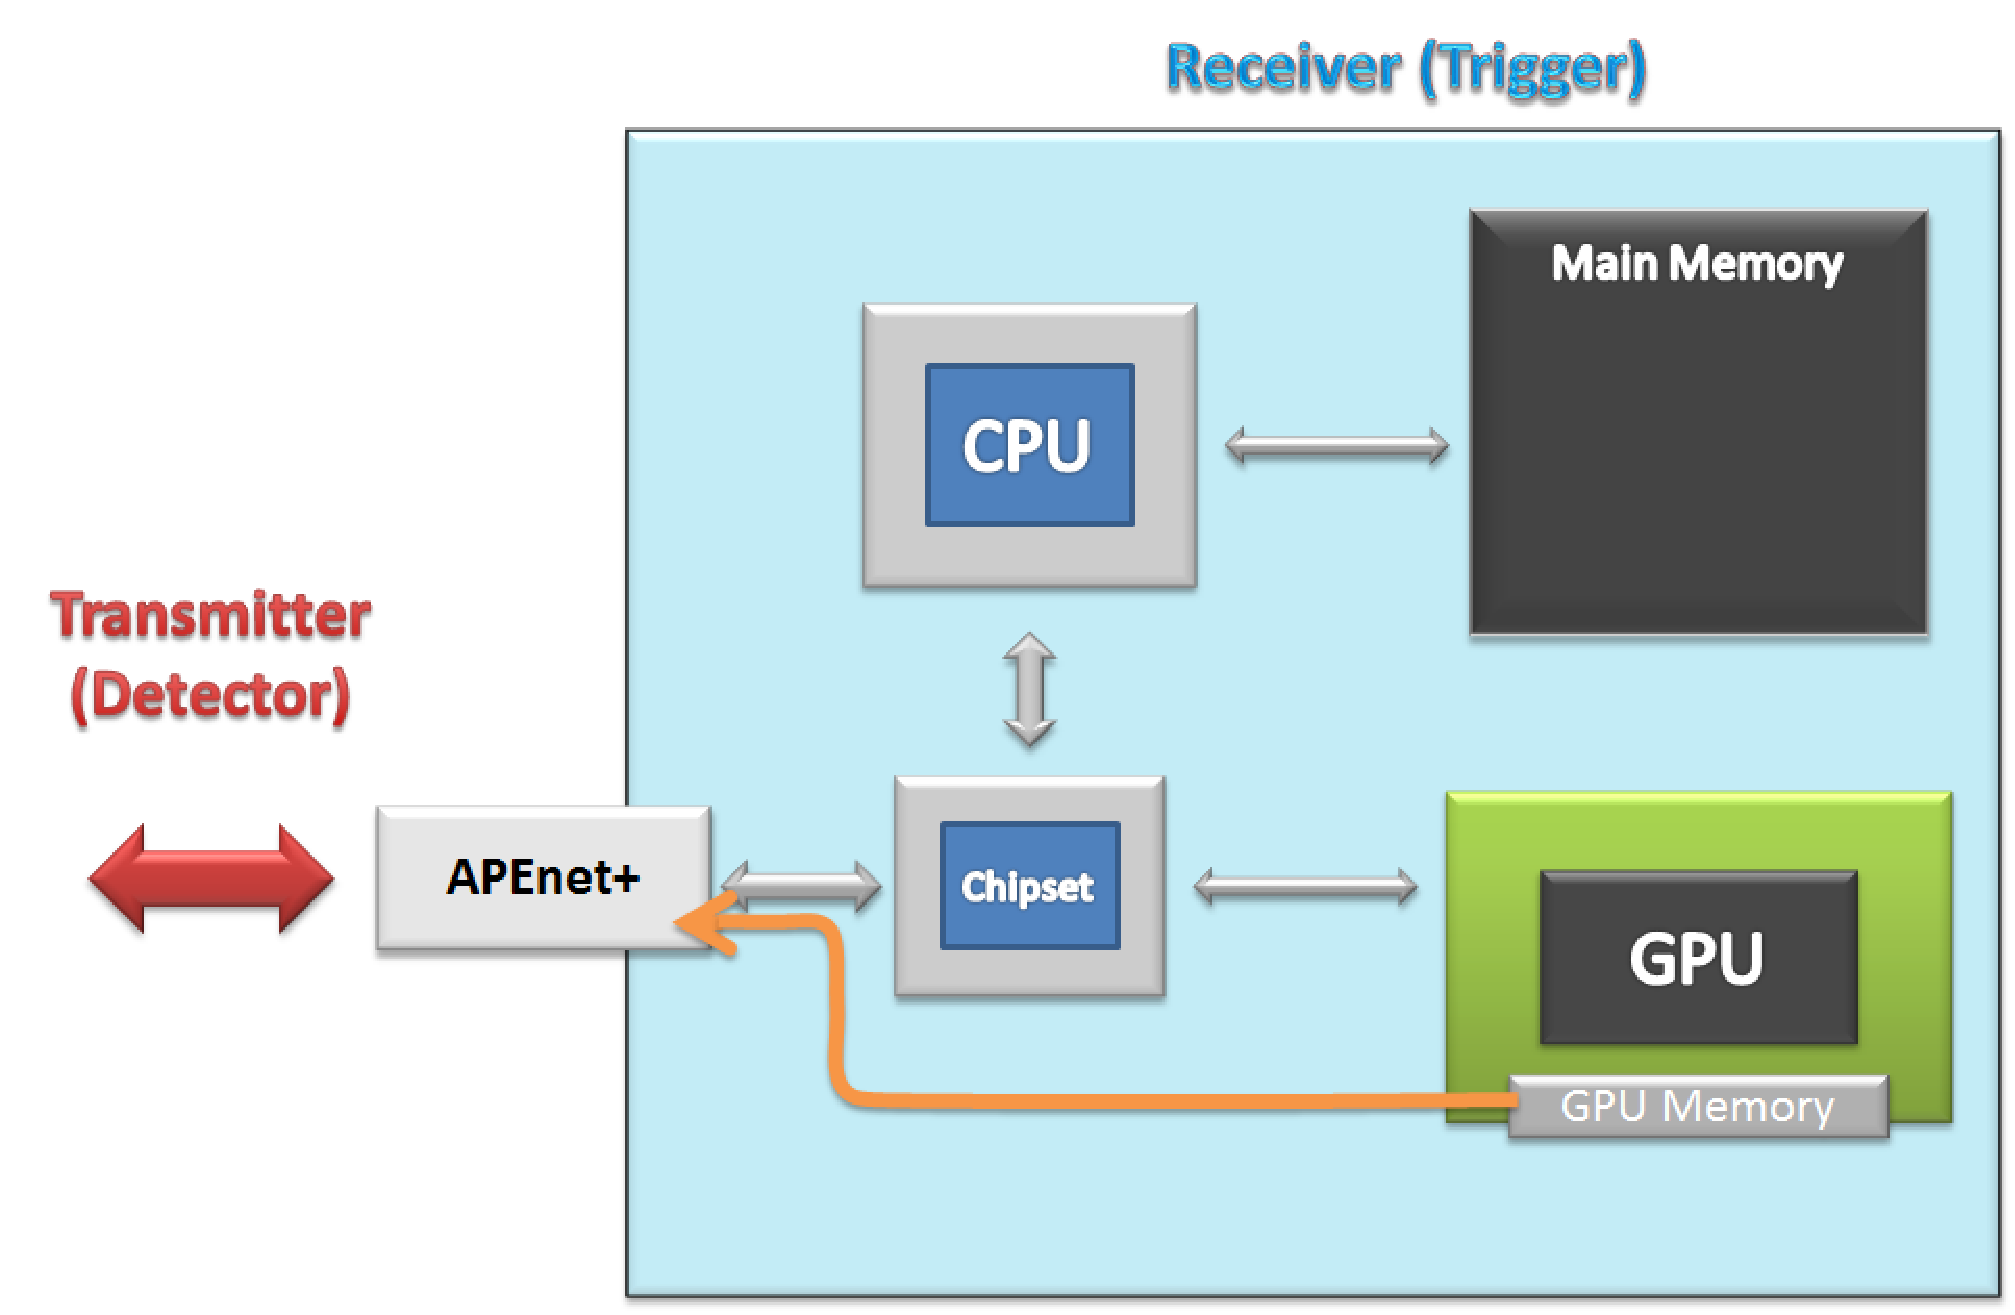
\includegraphics[width=0.3\linewidth]{figures/GPUDirect-APE}}
\caption{Standard data transfer (a), via GPUDirect (b) and via
  GPUDirect with P2P support (c). In (a), two buffers are required in
  the main memory. In GPUDirect (b), one of the main memory buffers is
  eliminated. In GPUDirect with P2P support, data is sent directly
  from the APEnet+ transceiver to the GPU memory.}
\end{figure*}

\begin{figure}[tbp]
  \centering
  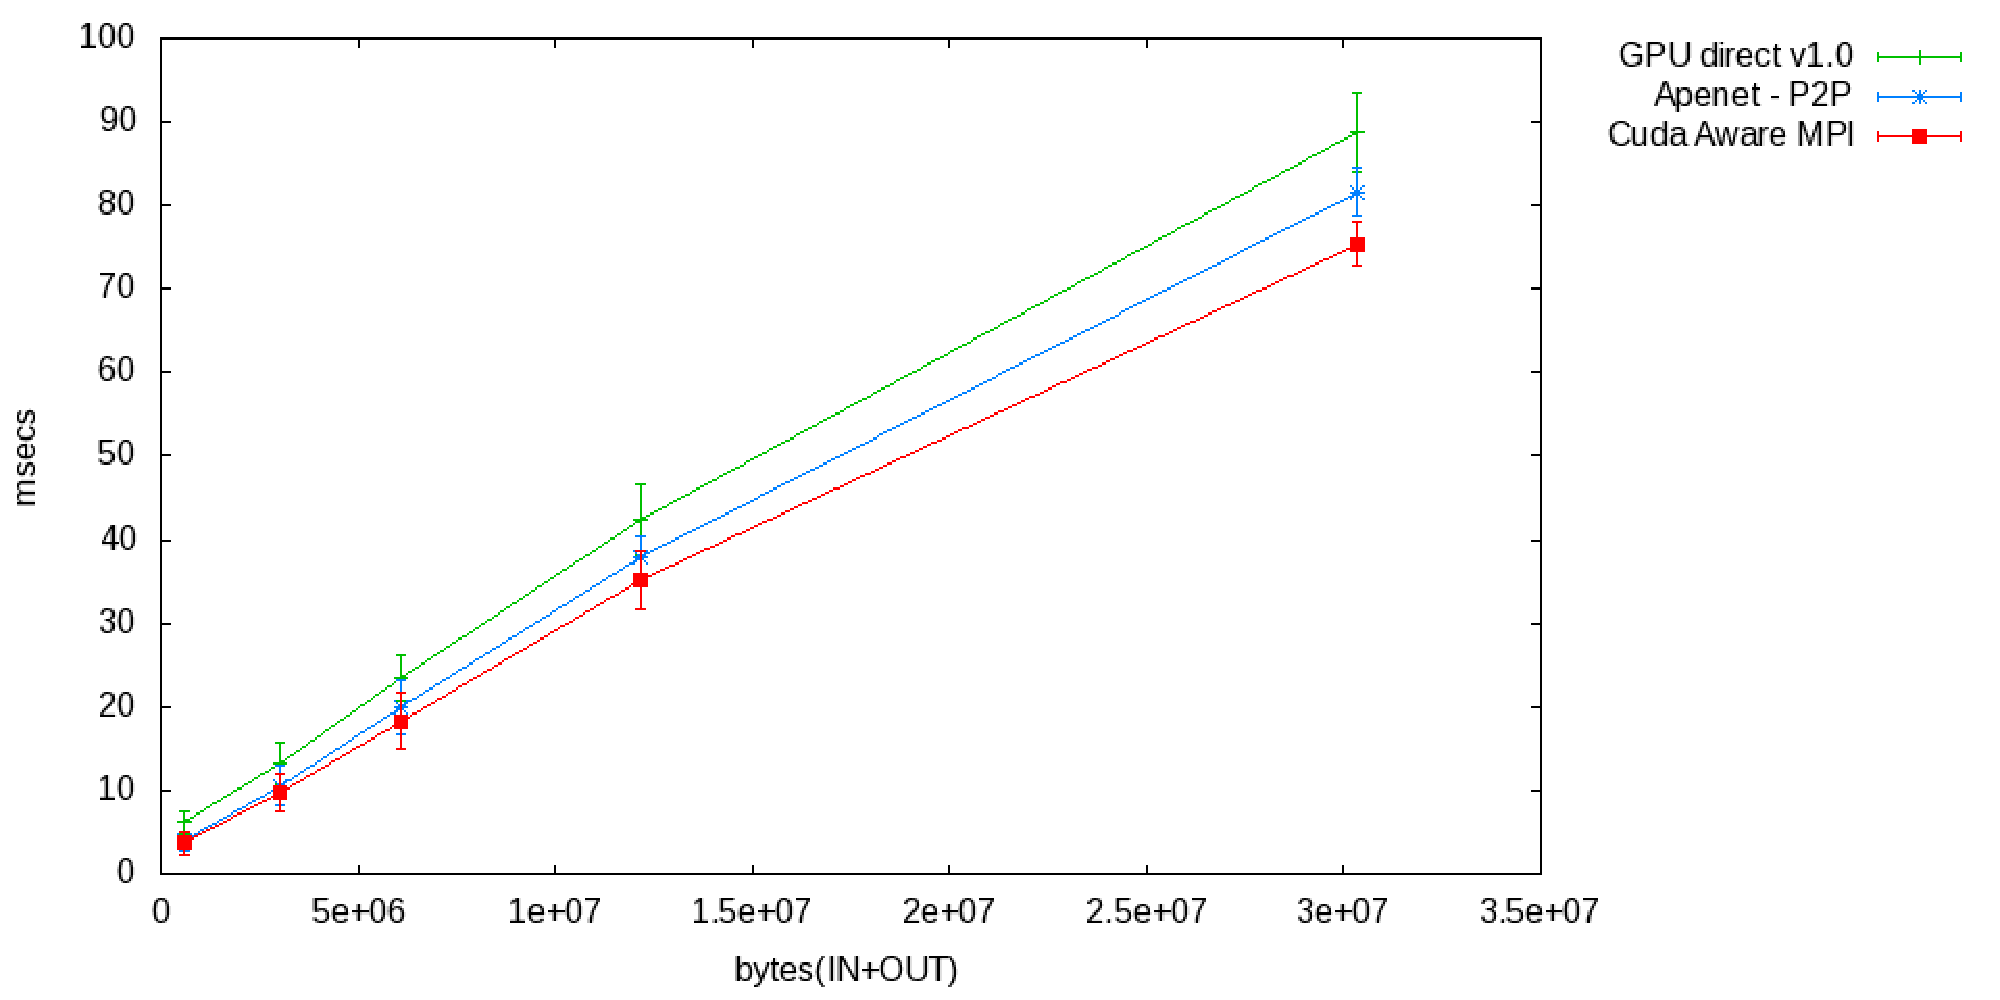
\includegraphics[width=0.9\linewidth]{figures/datatransfer.pdf}
  \caption{Total latency (data transfer, copy to/from the GPU and data processing on the GPU) as a function of data buffer sizes, for three different levels of optimization of GPUDirect: v1.0, CUDA-aware MPI and peer-to-peer. The smallest transferred data packed is 600 kB.}
  \label{fig:xferlatency}
\end{figure}

In Fig.~\ref{fig:xferlatency} we show the total latency (data transfer, copy to/from the GPU and data processing on the GPU) as a function of data packet size when data are transferred using GPUDirect v1.0,
CUDA-aware MPI and P2P. For the packet sizes over 600 kB CUDA-aware MPI gives the best performance.


\begin{figure}[tbp]
  \centering
  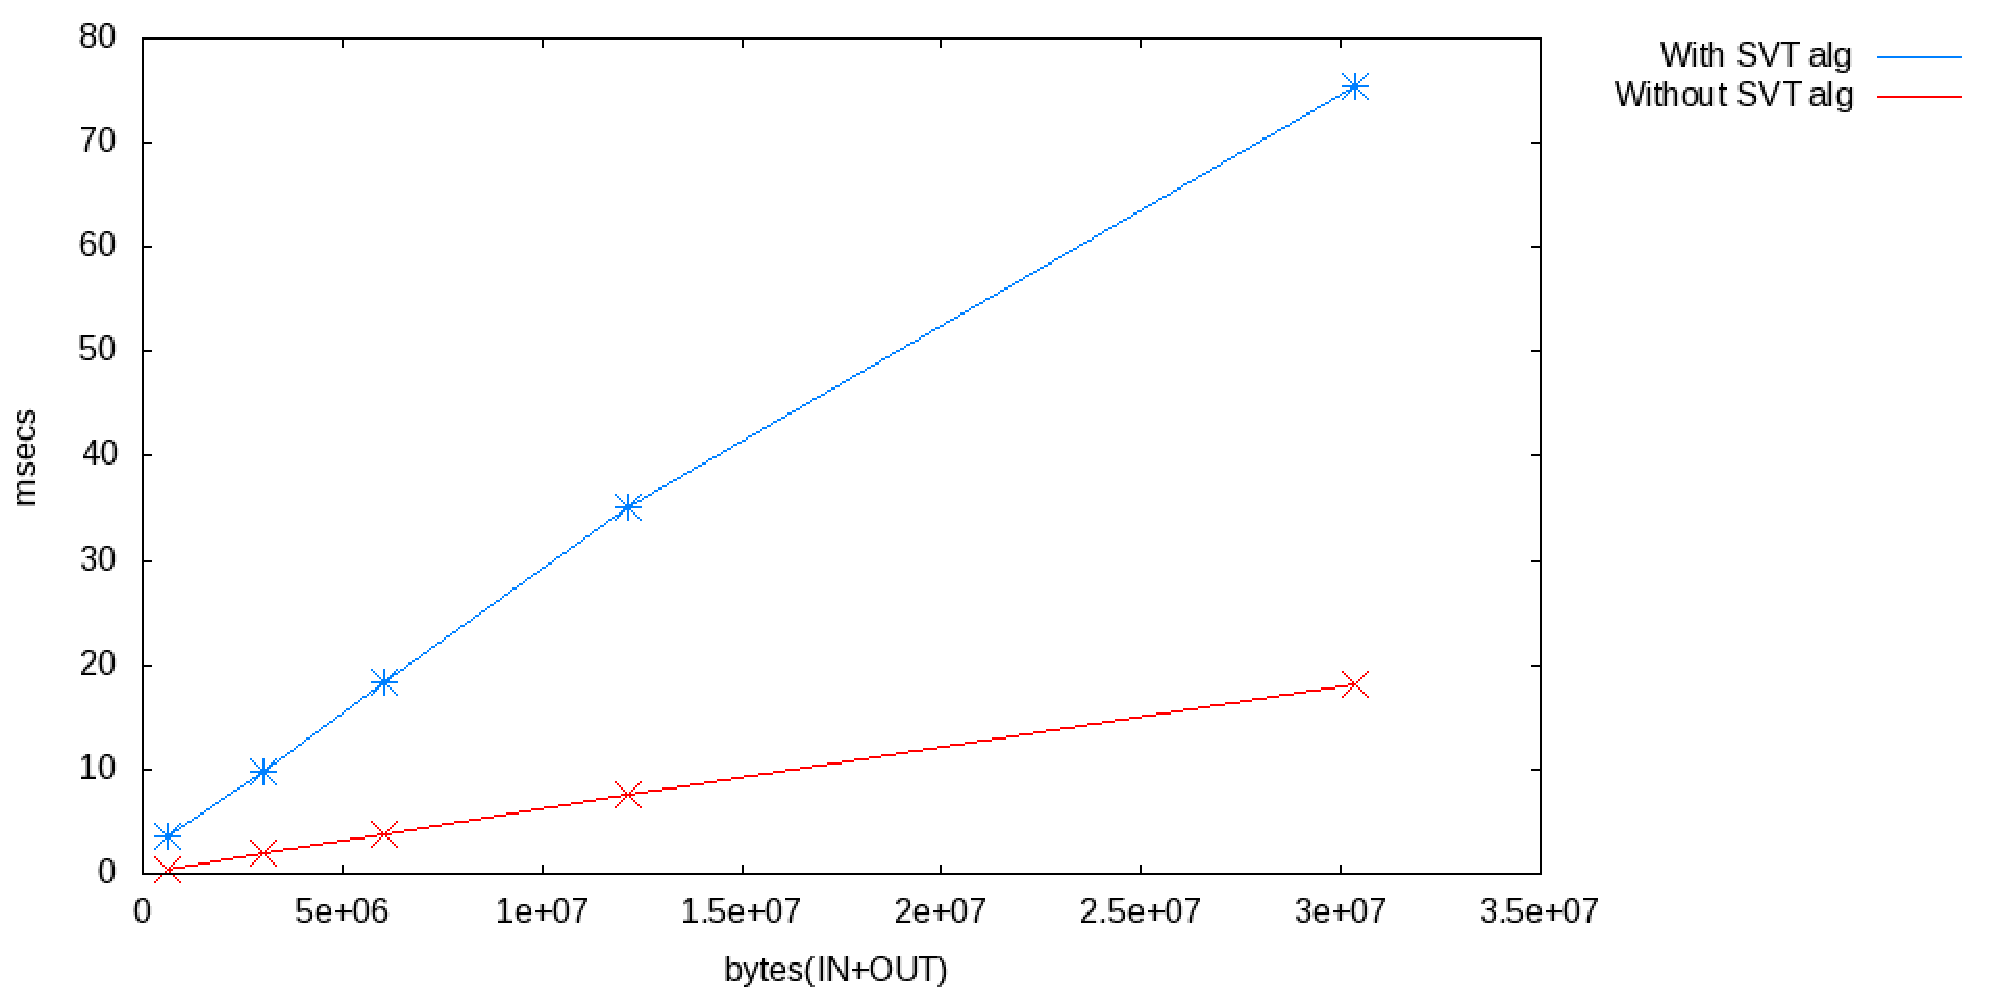
\includegraphics[width=0.9\linewidth]{figures/cudaware.pdf}
  \caption{data transfer latencies}
  \label{fig:transferOnly}
\end{figure}

The data transfer latency accounts for a significant part if the total latency, 
as can be seen in Fig.~\ref{fig:transferOnly}: about 20-25\% of total latency  is due to moving the data to and from the GPU.


\section{Conclusions}


%% gives unnumbered ack in CHEP style
\ack
The authors would like to thank the Fermilab staff and the FTK group at the 
University of Chicago for their support. This work was supported by the
U.S. Department of Energy, the U.S. National Science Foundation and the Italian
Istituto Nazionale di Fisica Nucleare. 

\section*{References}

%% CHEP2013 recommended style for bibliography
\bibliographystyle{iopart-num}

\bibliography{gpu}


% \bibitem{bib_cuda} \url{http://www.nvidia.com/object/cuda_home_new.html}

% \bibitem{bib_OpenCL} \url{http://www.khronos.org/opencl/}

% %\bibitem{bib_GPU_TIPP2011} Physics Procedia, Volume 37, 2012, 1965-1972.
% \bibitem{bib_Apenet} R.~Ammendola \textit{et al.}, \emph{APEnet+: a 3D toroidal network enabling Petaflops scale Lattice QCD simulations on commodity clusters}  PoS(Lattice 2010)022.


% \bibitem{bib_GPUDirect} \url{https://developer.nvidia.com/gpudirect}


 

\end{document}


